\documentclass{minimal}
\usepackage{tikz}
\usetikzlibrary{arrows,calc}
\tikzset{
%Define standard arrow tip
>=stealth',
%Define style for different line styles
help lines/.style={dashed, thick},
axis/.style={<->},
important line/.style={thick},
connection/.style={thick, dotted},
}
\begin{document}
  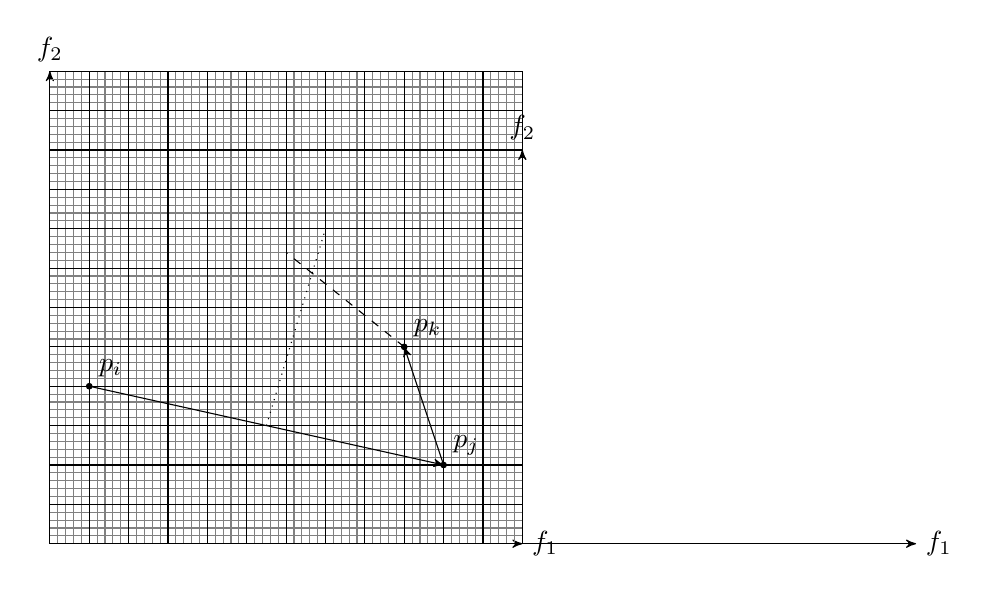
\begin{tikzpicture}[scale=1]

    % axis
    \coordinate (y) at (0,6);
    \coordinate (x) at (6,0);
    \draw[<->] (y) node[above] {$f_2$} -- (0,0) --  (x) node[right] {$f_1$};
    % A grid can be useful when defining coordinates
    \draw[step=1mm, gray, thin] (0,0) grid (6,6); 
    \draw[step=5mm, black] (0,0) grid (6,6); 

    % vectors
    \draw[->] (0.5,2) -- (5,1);
    \draw[->] (5,1) -- (4.5,2.5);

    % vectors' points
    \filldraw[black] (0.5,2) circle (1pt) node[above right,black] {$p_i$};
    \filldraw[black] (5,1) circle (1pt) node[above right,black] {$p_j$};
    \filldraw[black] (4.5,2.5) circle (1pt) node[above right,black] {$p_k$};

    % bissetriz
    \draw[dotted] (2.75, 1.5) -- (3.5,4.0);

    % distancia de p_k à bissetriz
    \draw[dashed] (4.5,2.5) -- (3.,3.7);

     % We start the second graph
     \begin{scope}[xshift=6cm]
       % Axis
      \coordinate (y2) at (0,5);
      \coordinate (x2) at (5,0);
      \draw[axis] (y2) node[above] {$f_2$} -- (0,0) --  (x2) node[right] {$f_1$};
      \end{scope}
    \end{tikzpicture}
  \end{document}
